%-------------------------
% Modern Professional Resume
% Author: Milav Jayeshkumar Dabgar
% Compiled with XeLaTeX for best results
%-------------------------

\documentclass[11pt,a4paper]{article}

% Packages for XeLaTeX
\usepackage{fontspec}
\usepackage{xunicode}
\usepackage{xltxtra}

% Modern fonts - Using simple font specification
\setmainfont{Times New Roman}
\setsansfont{Arial}

% Packages
\usepackage[margin=0.75in]{geometry}
\usepackage{xcolor}
\usepackage{titlesec}
\usepackage{enumitem}
\usepackage{multicol}
\usepackage{graphicx}
\usepackage{fontawesome5}
\usepackage{hyperref}
\usepackage{tikz}
\usepackage{array}
\usepackage{tabularx}

% Colors
\definecolor{primary}{RGB}{0, 79, 144}
\definecolor{secondary}{RGB}{64, 64, 64}
\definecolor{accent}{RGB}{0, 122, 204}
\definecolor{lightgray}{RGB}{245, 245, 245}

% Hyperref setup
\hypersetup{
    colorlinks=true,
    linkcolor=primary,
    urlcolor=primary,
    pdfauthor={Milav Jayeshkumar Dabgar},
    pdftitle={Resume - Milav Jayeshkumar Dabgar}
}

% Remove page numbers
\pagestyle{empty}

% Custom section formatting
\titleformat{\section}
    {\color{primary}\Large\sffamily\bfseries}
    {}
    {0em}
    {}[\color{primary}\titlerule]

\titleformat{\subsection}
    {\color{secondary}\large\sffamily\bfseries}
    {}
    {0em}
    {}

% Custom commands
\newcommand{\resumeItem}[1]{
    \item\small{#1 \vspace{-2pt}}
}

\newcommand{\resumeSubheading}[4]{
    \vspace{-1pt}\item
    \begin{tabular*}{0.97\textwidth}[t]{l@{\extracolsep{\fill}}r}
        \textbf{#1} & #2 \\
        \textit{\small#3} & \textit{\small #4} \\
    \end{tabular*}\vspace{-5pt}
}

\newcommand{\resumeProjectHeading}[2]{
    \vspace{-1pt}\item
    \begin{tabular*}{0.97\textwidth}{l@{\extracolsep{\fill}}r}
        \small#1 & #2 \\
    \end{tabular*}\vspace{-5pt}
}

\newcommand{\resumeSubItem}[1]{\resumeItem{#1}\vspace{-4pt}}

\renewcommand\labelitemii{$\vcenter{\hbox{\tiny$\bullet$}}$}

\newcommand{\resumeSubHeadingListStart}{\begin{itemize}[leftmargin=0.15in, label={}]}
\newcommand{\resumeSubHeadingListEnd}{\end{itemize}}
\newcommand{\resumeItemListStart}{\begin{itemize}}
\newcommand{\resumeItemListEnd}{\end{itemize}\vspace{-5pt}}

% Header design
\newcommand{\makeheader}{
    \begin{center}
        \begin{minipage}[t]{0.7\textwidth}
            \centering
            {\Huge\sffamily\bfseries\color{primary} Milav Jayeshkumar Dabgar}
            
            \vspace{5pt}
            {\Large\sffamily\color{secondary} Lecturer \& AI/Data Science Practitioner}
            
            \vspace{10pt}
            \begin{multicols}{2}
                \small
                \faIcon{envelope} \href{mailto:milav.dabgar@gmail.com}{milav.dabgar@gmail.com} \\
                \faIcon{phone} +91 8128576285 \\
                \faIcon{linkedin} \href{https://linkedin.com/in/milavdabgar}{linkedin.com/in/milavdabgar} \\
                \faIcon{globe} \href{https://milav.in}{milav.in} \\
                \faIcon{map-marker-alt} Gujarat, India \\
                \faIcon{id-card} AICTE Faculty ID: 1-3241967546
            \end{multicols}
        \end{minipage}
        \hfill
        \begin{minipage}[t]{0.25\textwidth}
            \raggedleft
            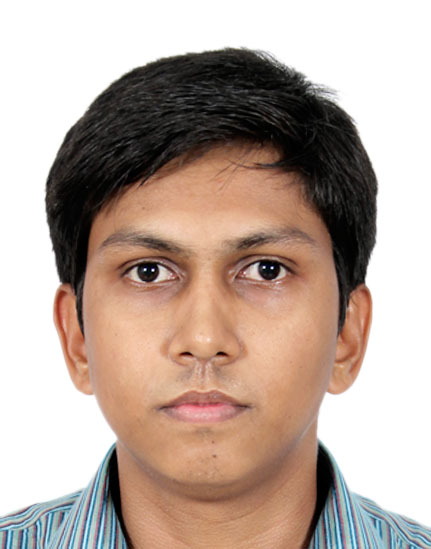
\includegraphics[width=3cm, height=3cm, keepaspectratio]{profile-picture.jpg}
        \end{minipage}
    \end{center}
    \vspace{-10pt}
}

%-------------------------------------------
%%%%%%  RESUME STARTS HERE  %%%%%%%%%%%%%%%%%%%%%%%%%%%%
%-------------------------------------------

\begin{document}

\makeheader

%----------- SUMMARY -----------
\section{Professional Summary}
\small Engineering educator and R\&D professional with 9+ years of experience spanning electronics hardware development, embedded systems, AI/ML, and full-stack software engineering. Currently pursuing BS in Data Science and Applications from IIT Madras (Diploma in Programming completed, one project away from Diploma in Data Science). Passionate about bridging theory and practice through innovative teaching, student mentorship, and real-world system development. Proven track record in leading technical initiatives, infrastructure management, and fostering innovation in academic environments.

%----------- EXPERIENCE -----------
\section{Professional Experience}
\resumeSubHeadingListStart

\resumeSubheading
{Lecturer (Class - II)}{Nov 2016 -- Present}
{Government Polytechnic, Education Department - Government of Gujarat}{Palanpur, Gujarat}
\resumeItemListStart
\resumeItem{Conduct Lab and Lecture Sessions for Programming in C, Microprocessor \& Assembly Language Programming, Microcontroller, Embedded Systems, Circuit Design \& Tools, Consumer Electronics, Entrepreneurship \& Industrial Management}
\resumeItem{Serve as \textbf{IT Convener}, \textbf{SSIP Co-Convener}, \textbf{Training \& Placement Member}, and contribute to MIS and UDAYAM initiative teams}
\resumeItem{Mentored student project teams in IoT, drones, and embedded automation resulting in \textbf{two student patents}}
\resumeItem{Led student teams that secured over \textbf{Rs. 25 lakhs funding from Shark Tank India} and \textbf{Rs. 20 lakhs through government innovation support}}
\resumeItem{Initiated and currently leading development of \textbf{Next.js-based smart academic portal} with smart attendance tracking, assessment workflows, committee management, automated result processing, and real-time analytics}
\resumeItem{Manage self-hosted Linux server infrastructure with Dockerized services, CI/CD pipelines, and backup systems}
\resumeItemListEnd

\resumeSubheading
{Electronics and Communication Engineer (R\&D)}{Jul 2015 -- Oct 2016}
{TEXEG India Private Limited (Japan-based firm)}{Gandhinagar, Gujarat}
\resumeItemListStart
\resumeItem{Managed end-to-end electronics development for commercial embedded products}
\resumeItem{Performed circuit simulation, PCB design, firmware development, and control systems implementation}
\resumeItem{Designed and tuned controllers (PID, PI, Fuzzy logic) using Control System Toolbox-MATLAB}
\resumeItem{Provided complete embedded solutions for R\&D projects and product development}
\resumeItemListEnd

\resumeSubheading
{Project Intern}{Aug 2014 -- Jul 2015}
{eiTRA - eInfochips Training \& Research Academy Ltd}{Ahmedabad, Gujarat}
\resumeItemListStart
\resumeItem{Gained hands-on experience in embedded systems and research methodologies}
\resumeItemListEnd

\resumeSubHeadingListEnd

%----------- EDUCATION -----------
\section{Education}
\resumeSubHeadingListStart

\resumeSubheading
{BS in Data Science and Applications}{2022 -- Present}
{Indian Institute of Technology Madras}{Online}
\resumeItemListStart
\resumeItem{\textbf{Diploma in Programming} (Completed)}
\resumeItem{\textbf{Diploma in Data Science} (One project away from completion)}
\resumeItem{Completed over 100 online courses in AI/ML and Data Science}
\resumeItemListEnd

\resumeSubheading
{Master's Degree, Communication Systems Engineering}{2013 -- 2015}
{L.D College of Engineering}{Ahmedabad, Gujarat}

\resumeSubheading
{Bachelor's Degree, Electronics and Communication Engineering}{2009 -- 2013}
{Sal Institute of Technology and Engineering Research}{Gujarat}

\resumeSubHeadingListEnd

%----------- TECHNICAL SKILLS -----------
\section{Technical Skills}
\begin{itemize}[leftmargin=0.15in, label={}]
    \small{\item{
        \textbf{Programming Languages:} Python, R, C, Assembly Language, JavaScript, SQL \\
        \textbf{Web Technologies:} Next.js, React, Node.js, HTML/CSS, RESTful APIs \\
        \textbf{Infrastructure \& DevOps:} Linux Server Administration, Docker, CI/CD Pipelines, Git, Self-hosted Solutions \\
        \textbf{Data Science \& AI:} Machine Learning, Deep Learning, Computer Vision, Data Analytics, Statistical Modeling \\
        \textbf{Embedded Systems:} STM32, Microcontrollers, PCB Design, Circuit Simulation, Firmware Development \\
        \textbf{Tools \& Platforms:} MATLAB, Control Systems Toolbox, Image Processing, IoT Systems \\
        \textbf{Areas of Expertise:} Full-Stack Engineering, Educational Technology, Infrastructure Management
    }}
\end{itemize}

%----------- KEY PROJECTS -----------
\section{Key Projects \& Achievements}
\resumeSubHeadingListStart

\resumeProjectHeading
{\textbf{Smart Academic Portal} $|$ \emph{Next.js, React, Node.js, Docker, Linux}}{2023 -- Present}
\resumeItemListStart
\resumeItem{Led development of comprehensive academic management system with smart attendance tracking, assessment workflows, committee management, automated result processing, and real-time feedback analytics}
\resumeItem{Deployed using self-hosted Linux infrastructure with Dockerized services, CI/CD pipelines, and backup systems}
\resumeItem{Collaborative development with student contributions through Git version control}
\resumeItemListEnd

\resumeProjectHeading
{\textbf{Student Innovation Mentorship Program} $|$ \emph{IoT, Drones, Embedded Systems}}{2018 -- Present}
\resumeItemListStart
\resumeItem{Mentored student teams resulting in two patents and significant funding successes}
\resumeItem{Guided projects that secured Rs. 25+ lakhs from Shark Tank India and Rs. 20 lakhs government support}
\resumeItem{Focus areas: IoT automation, drone technology, and embedded system applications}
\resumeItemListEnd

\resumeSubHeadingListEnd

%----------- LEADERSHIP -----------
\section{Leadership \& Administrative Roles}
\begin{itemize}[leftmargin=0.15in, label={}]
    \small{\item{
        \textbf{IT Convener:} Leading institutional technology initiatives and infrastructure development \\
        \textbf{SSIP Co-Convener:} Student Startup and Innovation Policy implementation and coordination \\
        \textbf{Training \& Placement Member:} Institutional placement and training committee \\
        \textbf{MIS \& UDAYAM:} Active contributor to Management Information Systems and UDAYAM initiatives
    }}
\end{itemize}

%----------- CERTIFICATIONS -----------
\section{Certifications \& Awards}
\resumeSubHeadingListStart

\resumeProjectHeading
{Student Innovation Success}{2024 -- 2025}
\resumeItemListStart
\resumeItem{Teams mentored secured Rs. 45+ lakhs in funding (Shark Tank India + Government Support)}
\resumeItemListEnd

\resumeProjectHeading
{IIT Madras Achievements}{2022 -- Present}
\resumeItemListStart
\resumeItem{Diploma in Programming (Completed), pursuing Diploma in Data Science}
\resumeItem{100+ completed NPTEL courses in AI/ML, Data Science, and related fields}
\resumeItemListEnd

\resumeProjectHeading
{NPTEL Recognition}{2019}
\resumeItemListStart
\resumeItem{NPTEL DISCIPLINE STARS - Computer Science}
\resumeItem{NPTEL ENTHUSIASTS \& BELIEVERS}
\resumeItemListEnd

\resumeSubHeadingListEnd

%----------- PROFESSIONAL OBJECTIVES -----------
\section{Professional Objectives}
\small
\textbf{Short-term:} Pursuing AICTE Industry Fellowship to gain applied industrial research experience in AI, embedded computing, or system design \\
\textbf{Long-term:} PhD in AI, Embedded Computing, or System Design from premier institution; Contributing to diploma-level innovation ecosystem in Gujarat \\
\textbf{Vision:} Bridge industrial rigor with academic excellence to foster research-driven education and interdisciplinary collaboration

%----------- PUBLICATIONS -----------
\section{Publications}
\resumeSubHeadingListStart
\resumeProjectHeading
{Resisting Blind Steganalysis in Real Time Covert Communication}{}
\resumeSubHeadingListEnd

\end{document}
